% !TEX encoding = UTF-8 Unicode
% !TEX TS-program = xelatex
\chapter{圓}
		\begin{tikzpicture}

\coordinate (cTPt) at (3,4);
\coordinate (cOPt) at (0,0);
\coordinate (cAPt) at (-6,0);
\coordinate (cBPt) at (6,0);

\coordinate (cQPt) at (3.6,4.8);


\draw[ultra thick] (cTPt) circle (1);
%\draw[ultra thick] (cOPt) circle (6);

\draw [ultra thick,domain=0:180] plot ({6*cos(\x)}, {6*sin(\x)});

\draw [ultra thick,dashed,domain=0:180] plot ({4*cos(\x)}, {4*sin(\x)});
\draw [ultra thick,dashed,domain=0:180] plot ({4.5*cos(\x)}, {4.5*sin(\x)});
\draw [ultra thick] (cQPt) -- (cOPt);
\draw [ultra thick] (cAPt) -- (cQPt) -- (cBPt) circle;

\foreach \v/\u/\t in 
{cTPt/270/$T$,
    cAPt/270/$A$,
    cBPt/270/$B$,
    cQPt/45/$Q$,
    cOPt/225/$O$
}
{
    \draw[ultra thick,fill] (\v) circle (2pt);
    \node[label=\u:\t] at (\v){};
};			
% x軸 y 軸 axes
\draw[-{Stealth[scale=1.3,angle'=45]},semithick] (-7,0) -- (7,0) node[] {$x$};
\draw[-{Stealth[scale=1.3,angle'=45]},semithick] (0,-0.5)->(0,7)   node[above] {$y$};


\end{tikzpicture}

	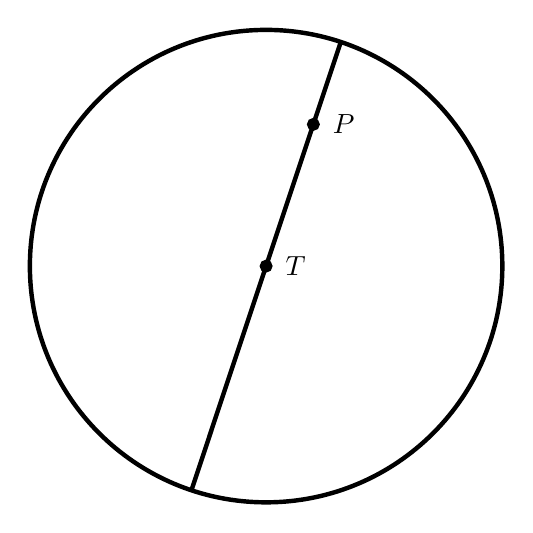
\begin{tikzpicture}[scale=0.3]
\coordinate (cPPt) at (3,4);	 
\coordinate (cTPt) at (1,-2);  

\draw[ultra thick] (cTPt) circle (10);

\draw[ultra thick,fill] (cTPt) circle (5pt);
\node[label=0:$T$] at (cTPt){};


\draw[ultra thick,fill] (cPPt) circle (5pt);
\node[label=0:$P$] at (cPPt){};
\begin{scope}[shift={(1,-2)}]
%劃出此題的直徑
\coordinate (cAPt) at (71.57:10);
\coordinate (cBPt) at (251.57:10);
\draw[ultra thick] (cAPt) -- (cBPt) ;	
\end{scope}  



\end{tikzpicture}

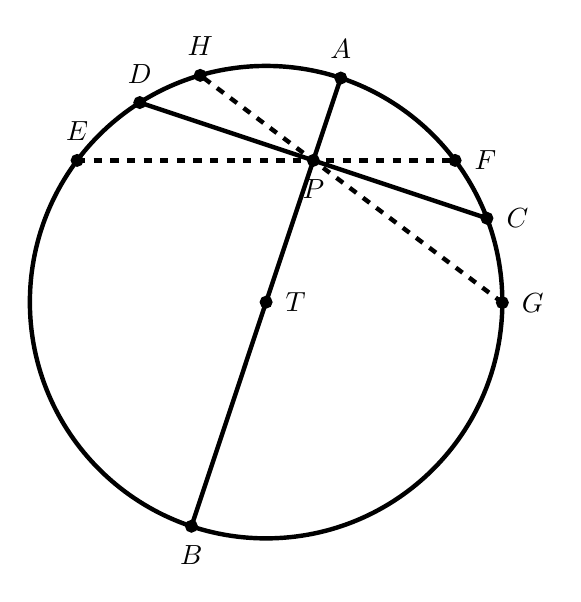
\begin{tikzpicture}[scale=0.3]
\coordinate (cPPt) at (3,4);	 
\coordinate (cTPt) at (1,-2);  

\draw[ultra thick] (cTPt) circle (10);

\draw[ultra thick,fill] (cTPt) circle (5pt);
\node[label=0:$T$] at (cTPt){};


%\draw[ultra thick,fill] (cPPt) circle (5pt);
%\node[label=0:$P$] at (cPPt){};

\begin{scope}[shift={(1,-2)}]
%劃出此題的直徑
\coordinate (cAPt) at (71.57:10);
\coordinate (cBPt) at (251.57:10);


\draw[ultra thick] (cAPt) -- (cBPt) ;	
\begin{scope}[shift={(2,6)}]
\coordinate (cCPt) at ({71.57-90}:{sqrt(60)});
\coordinate (cDPt) at ({71.57+90}:{sqrt(60)});
\draw[ultra thick] (cCPt) -- (cDPt) ;
\end{scope}
%	
\end{scope}

%%舉例 弦長為 16 的兩條對稱位置:
\coordinate (cEPt) at (-7,4);
\coordinate (cFPt) at (9,4);
\coordinate (cGPt) at (11,-2.02);
\coordinate (cHPt) at (-1.79,7.6);

\draw[ultra thick,dashed] (cEPt) -- (cFPt) ;	
\draw[ultra thick,dashed] (cGPt) -- (cHPt) ;

\foreach \v/\u/\t in 
{cAPt/90/$A$,
    cBPt/270/$B$,
    cCPt/0/$C$,
    cDPt/90/$D$,
    cEPt/90/$E$,
    cFPt/0/$F$,
    cGPt/0/$G$,
    cHPt/90/$H$,
    cPPt/270/$P$}
{
    \draw[ultra thick,fill] (\v) circle (5pt);
    \node[label=\u:\t] at (\v){};
};	

\end{tikzpicture}

    \begin{tikzpicture}[scale=0.7]
\newcommand{\nA}{0}
\newcommand{\nB}{10}
\coordinate (cAPt) at (\nA, 0);
\coordinate (cBPt) at (\nB, 0);
\draw [ultra thick](cAPt)--(cBPt);
\draw [ultra thick] (10,0) arc [radius=5, start angle=0, end angle= 180];
\node[label=180:$A$] at (cAPt){};
\node[label=0:$B$] at (cBPt){};

\coordinate (cA1Pt) at (1, 0);
\coordinate (cB1Pt) at (1, 3);
%\draw [ultra thick](cA1Pt)--(cB1Pt);
\coordinate (cA2Pt) at (2, 0);
\coordinate (cB2Pt) at (2, 4);
\coordinate (cA3Pt) at (3, 0);
\coordinate (cB3Pt) at (3, {sqrt(21)});
\coordinate (cA4Pt) at (4,0);
\coordinate (cB4Pt) at (4, {sqrt(24)});
\coordinate (cA5Pt) at (5,0);
\coordinate (cB5Pt) at (5,5);

\coordinate (cA6Pt) at (6,0);
\coordinate (cA7Pt) at (7,0);
\coordinate (cA8Pt) at (8,0);
\coordinate (cA9Pt) at (9,0);
\coordinate (cB6Pt) at (6,{2*sqrt(6)});
\coordinate (cB7Pt) at (7,{sqrt(21)});
\coordinate (cB8Pt) at (8,4);
\coordinate (cB9Pt) at (9,3);
\foreach \v/\u in {A1Pt/B1Pt,A2Pt/B2Pt, A3Pt/B3Pt, A4Pt/B4Pt, A5Pt/B5Pt, A6Pt/B6Pt, A7Pt/B7Pt, A8Pt/B8Pt, A9Pt/B9Pt}
{
    \draw [ultra thick](c\v)--(c\u);
};
\node[label=270:$A_1$] at (cA1Pt){};
\node[label=90:$B_1$] at (cB1Pt){};
\node[label=270:$A_2$] at (cA2Pt){};
\node[label=90:$B_2$] at (cB2Pt){};
\node[label=270:$A_9$] at (cA9Pt){};
\node[label=90:$B_9$] at (cB9Pt){};

\end{tikzpicture}

    \begin{tikzpicture}[scale=1.5]
\coordinate (cOPt) at (0:0);
%    \coordinate (cAPt) at (0:1);
%    \coordinate (cBPt) at (56:1);	%粗略B值
%    \coordinate (cCPt) at (112:1);	%粗略C值
\coordinate (cPPt) at (1,-1);
\coordinate (cQPt) at (-1.37,-0.37);
\coordinate (cRPt) at (0.37,1.37);
\coordinate (cHPt) at (-0.5,0.5);
%H = (-0.5, 0.5)
%P = (1, -1)
%Q = (-1.37, -0.37)
%R = (0.37, 1.37)

\draw [ultra thick](cPPt) --(cQPt) -- (cRPt) -- (cPPt) circle;

\draw [ultra thick](cPPt) --(cHPt) ;
\draw [ultra thick](cOPt) --(cRPt) ;

\draw[ultra thick] (cPPt) circle (1pt);
\draw[ultra thick] (cQPt) circle (1pt);
\draw[ultra thick] (cRPt) circle (1pt);

\draw[domain=-1.7:0.7,smooth,variable=\x,ultra thick] plot ({\x},{\x+1});

\draw[ultra thick] (0,0) circle ({sqrt(2)});

\node[label=225:$O$] at (cOPt){};
\node[label=0:$P$] at (cPPt){};
\node[label=180:$Q$] at (cQPt){};
\node[label=90:$R$] at (cRPt){};
\node[label=135:$H$] at (cHPt){};
\node at (1.8,1.6){$x-y+1=0$};

% x軸 y 軸 axes
\draw[-{Stealth[scale=1.3,angle'=45]},semithick] (-2,0) -- (2,0) node[] {$x$};
\draw[-{Stealth[scale=1.3,angle'=45]},semithick] (0,-2)->(0,2)   node[above] {$y$};
\end{tikzpicture}


\begin{tikzpicture}[line cap=round,line join=round,x=0.7cm,y=0.7cm]
\draw[-{Stealth[scale=1,angle'=45]},color=black] (-5,0.) -- (4,0.)  node[] {$x$};
%\foreach \x in {-3,-2,-1,1,2}
%\draw[shift={(\x,0)},color=black] (0pt,2pt) -- (0pt,-2pt) node[below] {\footnotesize $\x$};
\draw[-{Stealth[scale=1,angle'=45]},color=black] (0.,-7.5) -- (0.,2) node[above] {$y$};
%    \foreach \y in {1,2}
%    \draw[shift={(0,\y)},color=black] (2pt,0pt) -- (-2pt,0pt) node[left] { $\y$};
%    


\draw(-0.5,-2.5) circle (3.535);

\draw[ultra thick,fill] (-3,0) circle (0.8pt) node [ above left] {$P(k,0)$};
\draw[ultra thick,fill] (2,0) circle (0.8pt) node [ above ] {$Q(2,0)$};
\draw[ultra thick,fill] (0,1) circle (0.8pt) node [ above ] {$R(0,1)$};

\end{tikzpicture}